%%=============================================================================
%% Methodologie
%%=============================================================================

\chapter{\IfLanguageName{dutch}{Methodologie}{Methodology}}
\label{ch:methodologie}

%% TODO: Hoe ben je te werk gegaan? Verdeel je onderzoek in grote fasen, en
%% licht in elke fase toe welke stappen je gevolgd hebt. Verantwoord waarom je
%% op deze manier te werk gegaan bent. Je moet kunnen aantonen dat je de best
%% mogelijke manier toegepast hebt om een antwoord te vinden op de
%% onderzoeksvraag.

In dit stuk van de bachelorproef zal men uitleggen hoe het onderzoek tot stand heeft gebracht. Men kan hierin waarnemen hoe men beslissingen heeft genomen omtrent specifieke eigenschappen van de verschillende AI-frameworks. Dit hoofdstuk is verdeeld is vier subsecties, elk van hen verdiept zich meer in hoe elk bepaald stuk van het onderzoek werd gerealiseerd.

\section{Voorbereiding}
Deze subsectie verdiept zich in hoe het toekomstig onderzoek werd uitgestippeld. Men ging verschillende toenaderingen zoeken om een AI-framework op een zo goed mogelijke manier te kunnen evalueren, dit is vervolgens het raamwerk dat werd gebruikt als aanpak in de evaluatie. Er werd ook een extra exploratief onderzoek verwezenlijkt om reeds uitgewerkte voorbeelden te achterhalen die gebruikt maakten van de concrete AI-frameworks. Op deze manier kon men snel testen of de frameworks de moeite waard zijn om deze verder te gebruiken in de proof-of-concept.
\newpage

\subsection{ Onderzoek naar AI-frameworks}
Bij het zoeken van de verschillende frameworks heeft men rekening gehouden met bepaalde criteria die invloed zouden kunnen hebben op het onderzoek:
\begin{itemize}
	\item De kost van het framework (betalend of gratis)
	\item Een mogelijke limiet op het aantal 'calls'
	\item De compatibiliteit met ARKit
	\item Documentatie
	\item Reeds uitgewerkte voorbeelden
\end{itemize}

In dit onderzoek werden 2 AI-frameworks onder de loep genomen, deze voldeden reeds aan alle criteria die werden opgesteld:

\begin{itemize}
	\item TensorFlow Lite (TensorFlow)
	\item CoreML (Apple)
\end{itemize}

De twee andere frameworks die ook werden besproken in de stand van zaken werden niet onderzocht, deze frameworks zijn immers betalend (Vuforia en Vision API). 

\subsection{Beoordelingstechnieken}
Om het juiste AI-framework te kiezen heeft men elk van hen op een grondige manier geëvalueerd. Om dit op een optimale manier te doen heeft men rekening gehouden met verschillende beoordelingstechnieken.

\subsubsection{Functionaliteit}
De eerste factor waar men rekening mee heeft gehouden is het feit of het AI-framework wel degenlijk deed wat er gevraagd werd. Om de frameworks op een zo divers mogelijk manier te kunnen testen heeft men verschillende soorten AI-eigenschappen getest:
\begin{itemize}
	\item Objectdetectie
	\item Menssegmentatie
	\item Luchtsegmentatie 
	\item Segmentatie binnen gebouwen
\end{itemize}
Segmentatie is het opsplitsen van een bepaald beeld in verschillende segmenten. Op deze manier zou het AI-framework bijvoorbeeld muren en grond van elkaar kunnen onderscheiden. De combinatie van objectdetectie en segmentatie is van zeer groot belang binnen deze bachelorproef, zo kan men vervolgens verschillende soorten objecten van elkaar onderscheiden en bepalen waar die zich juist bevinden. Deze uitvoering werd reeds uitgewerkt door 'Gestalt Robotics', een robot zal door deze implementatie op een correctie manier door het fabrieksgebouw bewegen.

\begin{figure}[H]
	\centering
	\includegraphics[scale=0.3]{SemanticSegmentation_ObjectDetection.png}
	\caption{Voorbeeld segmentatie + objectdetectie \autocite{Gestalt2019}}
\end{figure}

\subsubsection{Correctheid}
De 2de en meest cruciale factor is de correctheid van het AI-framework voor de verschillende soorten AI-eigenschappen. Het is belangrijk dat het framework betrouwbaar is en dus geen foute oplossing zal terug geven, anders zal dit verkeerd doorgegeven worden aan de visuele kant van de applicatie en zal de route verkeerd worden aangegeven. Om de correctheid van elk AI-framework te testen heeft men opnieuw de diverse AI-eigenschappen onder de loep genomen.

\subsubsection{Correctheid - 1.  Objectdetectie}
Om de objectdetectie te evalueren heeft men geobserveerd of het framework de juiste positie van het gerelateerde object aangeeft , alsook het percentage dat de correctie voorstelt werd in acht gehouden.

\subsubsection{Correctheid - 2. Menssegmentatie}
Bij de evaluatie van de menssegmentatie werd er gekeken of het computer gegenereerde oppervlak overeen kwam met de vorm van de daadwerkelijke persoon. De foute zones werden aangeduid met markeringen om een duidelijk overzicht te krijgen.

\subsubsection{Correctheid - 3. Luchtsegmentatie}
Luchtsegmentatie werd op dezelfde manier beoordeeld als menssegmentatie. Deze twee segmentaties hebben een zeer gelijkaardige input en output, maar toch is er een groot verschil binnenin het framework. Het algoritme wordt op een andere manier getraind en zo is er toch een mogelijkheid dat deze twee segmentaties voor verschillende resultaten zorgen.

\subsubsection{Correctheid - 4. Segmentatie binnen gebouwen}
Segmentatie binnen gebouwen is de uitwerking die het meest gerelateerd is met de AI-output die voor deze bachelorproef van belang is. Het biedt namelijk de mogelijkheid om muren van grond te onderscheiden, dit is de hoofdreden waarom men AI in deze wayfinding-uitwerking wilt betrekken. Het is dus belangrijk dat deze AI-uitwerking grondig wordt geëvalueerd.

De evaluatie verliep als volgt, voor beide AI-frameworks werd op identiek dezelfde plaats de test uitgevoerd. De resultaten werden naast elkaar geplaatst en vervolgens geëvalueerd door de foute zones aan te duiden, ook werd er gekeken naar de extra info die men kon vergaren uit beide resultaten. Het framework die het best de verschillende soorten segmenten kon 'vertellen', werd gezien als beste framework in deze sectie.

\begin{figure}[H]
	\centering
	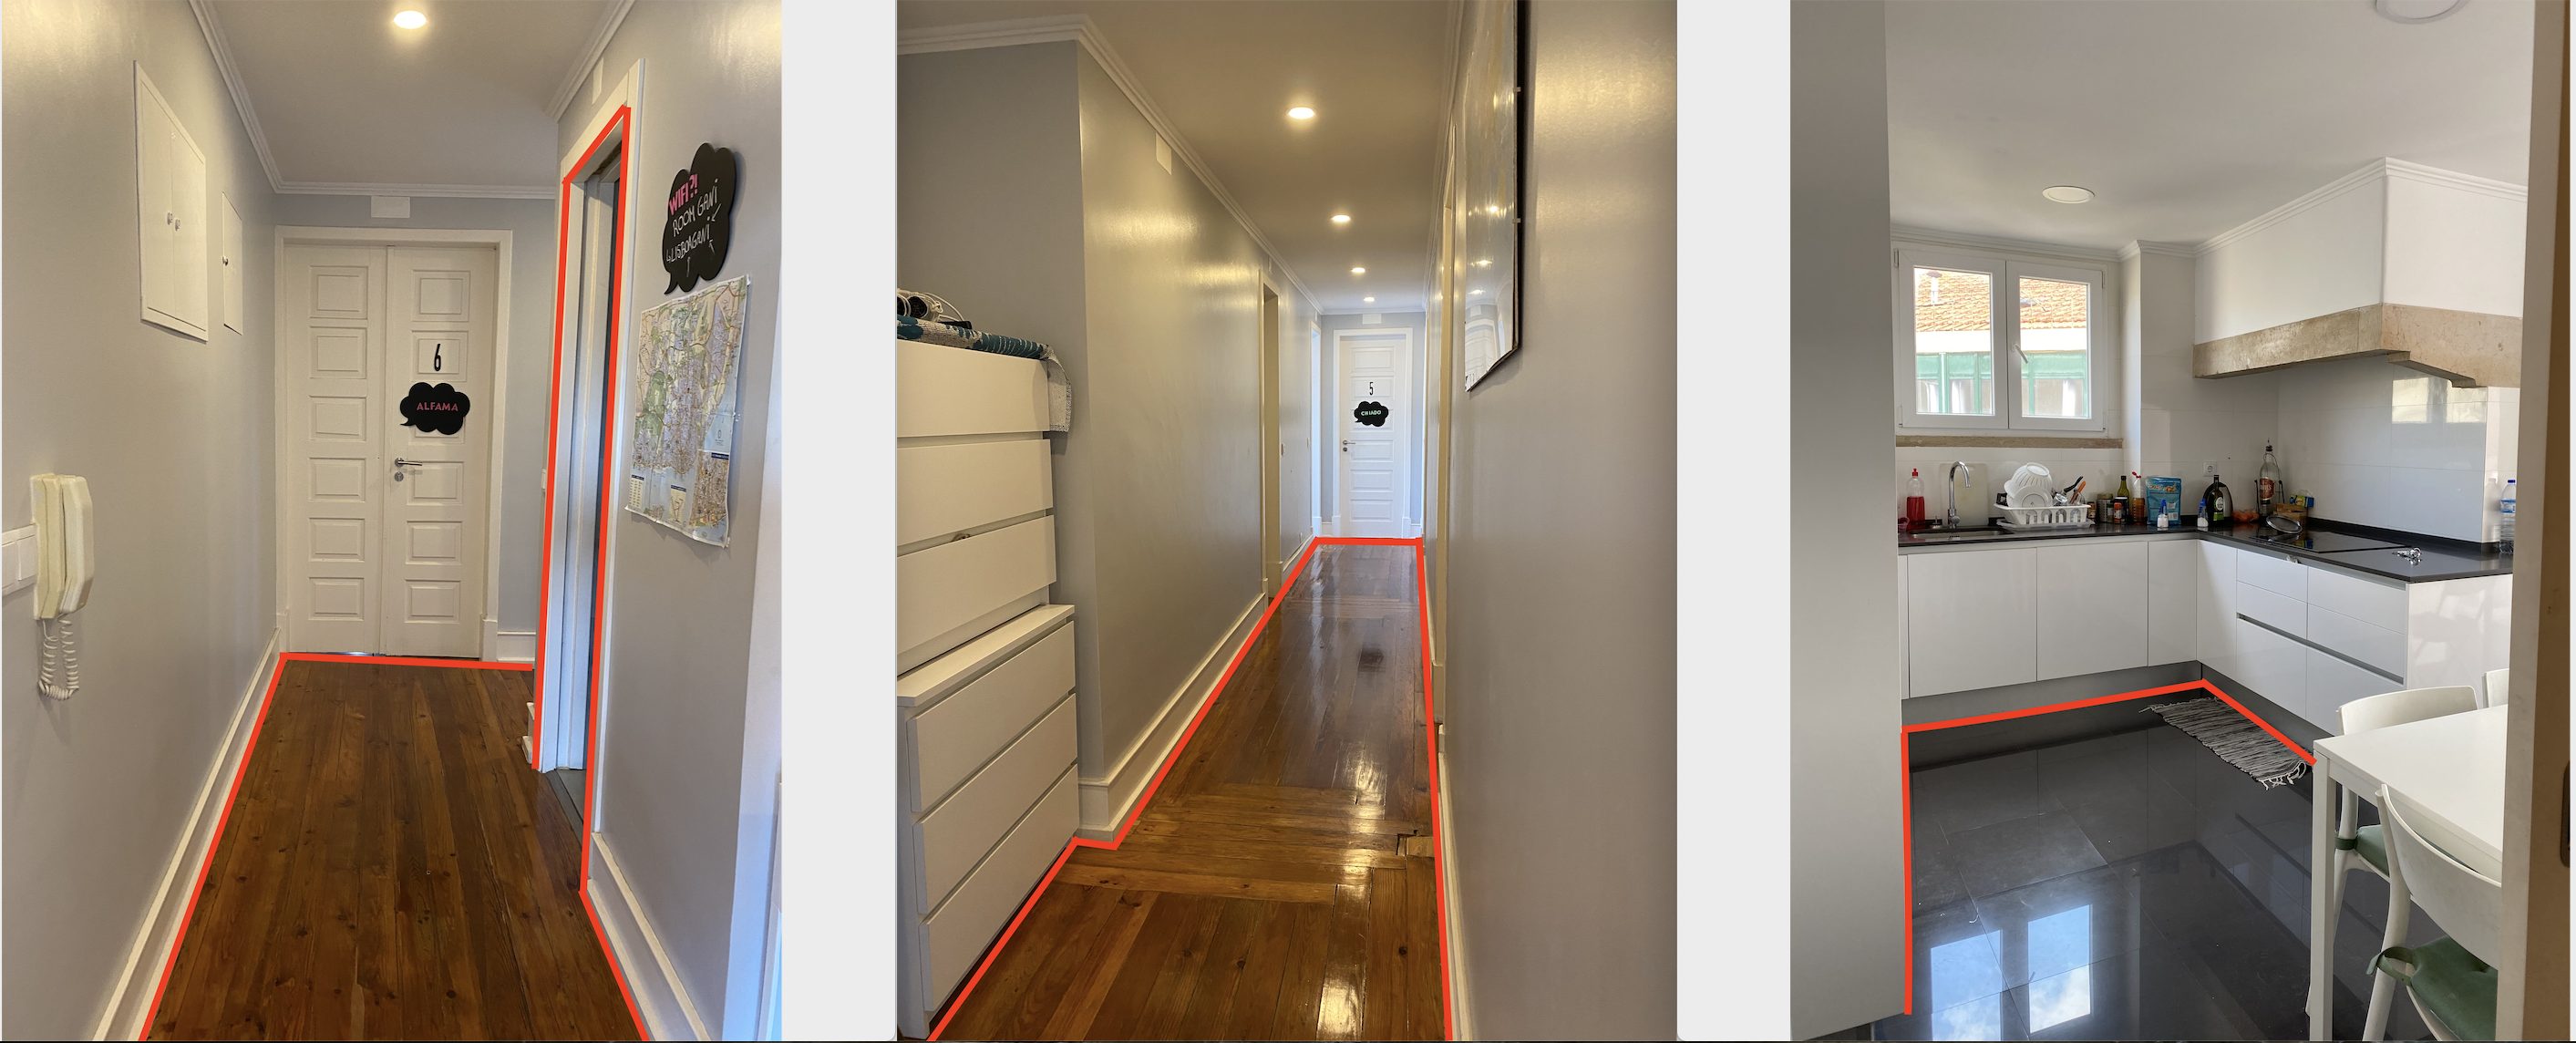
\includegraphics[scale=0.3]{BeoordelingsTechnieken.png}
	\caption{Voorbeeld evaluatietechniek segmentatie binnen gebouwen}
\end{figure}

\subsubsection{Toegankelijkheid}
Een tweede belangrijke factor is de toegelankelijkheid van de AI-frameworks voor verschillende platformen. Zo is het belangrijk voor het bedrijf 'In The Pocket' dat ze een oplossing vinden dat schaalbaar is.

\subsection{Bepalen van optimaal AI-framework}
Het bepalen van welk AI-framework de optimale oplossing biedt werd gemaakt op basis van een overzicht van alle testen. Dit overzicht bevat staafdiagrammen die de resultaten van alle testen in kaart brengt, zo kan men rekening houden met de verschillende eigenschappen die elk framework te bieden heeft.

\section{Evaluatie}

\section{Resultaten}

